% \subsection{OpenTelemetry}
% \label{subsec:opentelemetry}

Auf Basis dieser der drei Grundpfeiler Logging, Metriken und Tracing haben sich einige Technologien entwickelt. Viele dieser Ansätze sind proprietär und nicht miteinander kompatibel, weswegen das Bedürfnis einer Standardisierung entstand. Um die hier angesiedelten Technologien zu vereinheitlichen enstanden u. A. OpenTracing, OpenCensus \cite{OpenCensus} sowie OpenTelemetry \cite{OpenTelemetry}, die jeweils darauf abzielen herstellerunabhängige Observability-Konzepte zu definieren.

OpenTelemetry (OTel) ist ein sich derzeit\footnote{Ein erster (General-Availability-)Release der Spezifikation ist für die erste Hälfte 2021 geplant \cite{OpenTelemetryGARelease} (Stand 01.03.2021)} entwickelnder Standard, welcher als Ziel hat, das Erfassen, Weiterleiten und Verarbeiten von Tracing-, Metrik- und Logdaten\footnotemark{} herstellerunabhängig zu ermöglichen. OTel entwickelte sich aus dem Zusammenschluss der Teams hinter den beiden Standards OpenTracing und OpenCensus  \cite{UseNixDistributiveTracing}. Microsoft, Google, führende Unternehmen und Entwickler von Observability-Technologien sowie die Cloud-Native-Computing-Foundation (CNCF) arbeiten an der Entwicklung des OTel-Standards \cite{DistributedTracingInPractice} \cite{OpenTelemetryCommunityMembers}. OTel versucht nicht nur die bisherige Landschaft zu vereinigen, sondern definiert eine zukunftsorientierte Architektur, die aus unterschiedlichen Komponenten besteht und definiert, wie diese miteinander kommunizieren \cite{DistributedTracingInPractice}.

\nomenclature[Fachbegriff]{OTel}{OpenTelemetry}
\nomenclature[Fachbegriff]{CNCF}{Cloud-Native-Computing-Foundation}
\footnotetext{Die Entwicklung einer Logging-Spezifikation ist im Gange \cite{OpenTelemetryLoggingSpecification}.}

Der OpenTelemetry-Standard definiert einige Komponenten, die spezielle Aufgabengebiete abdecken und standardisiert mit anderen Komponenten kommunizieren. Diese Komponenten werden nachfolgend anhand des Beispiels eines Tracing-Spans sowie der \autoref{fig:otel-components} erläutert.

\begin{itemize}
	\item \textbf{API}: Die API stellt die öffentlich sichtbare Schnittstelle der \enquote{low-level} OTel-Verarbeitung (des SDKs) dar, die Zielgruppe umfasst Entwickler sowie instrumentierende Bibliotheken. Mit der API kann ein Entwickler einen Trace initialisieren, darauf aufbauend einen Span erzeugen und diesen Span starten.
	
	\item \textbf{Instrumentation-Library}: Bei dieser Bibliothek handelt es sich um eine spezifische Anbindung der OTel-API bspw. an ein Framework (wie JAX-RS oder Angular). Teilweise erlauben solche Bibliotheken auch eine automatische Erfassung der Daten, sodass bei relevanten Methoden (wie Schnittstellaufrufen) ein Span erzeugt wird.
	
	\item \textbf{SDK}: Das SDK stellt das Herzstück der Logik bei OTel dar und beinhaltet die interne Verarbeitung der Daten. Ein erzeugter Span wird hier mit seinen Kontextinformationen zwischengespeichert und bei Beendigung des Spans wird dieser an angebundene Exporter übergeben.
	
	\item \textbf{Exporter}: Exporter sind spezifische Anbindungen, welche Daten im OTel-Format annehmen und für Gegenstellen aufbereiten und an diese transportieren. Die Gegenstelle kann entweder eine Datensenke darstellen oder auch eine weiterverarbeitende Komponente sein. Im Beispiel (vgl. \autoref{fig:otel-components}) wird der Span nicht in ein anderes Format überführt, da er an einen OTel-Colletor gesendet wird.
	
	\item \textbf{Collector}: Kollektoren sind eine OTel-Schnittstelle, um unterschiedliche OTel-Daten anzunehmen und diese an weitere Systeme mithilfe von Exportern zu übergeben. Bei dem Exporter in diesem Beispiel werden die Daten in das passende Format des Telemetry-Backends überführt.
	
	\item \textbf{Telemetry-Backend}: Ein Telemetry-Backend stellt die Datensenke der OTel-Daten dar und bietet den Entwicklern und Betreibern eine Visualisierung der gesammelten Daten. Beispiele hierfür sind z. B. Jaeger \cite{Jaeger} oder Prometheus \cite{Prometheus}.
\end{itemize}
 
\begin{figure}[H]
	\centering
	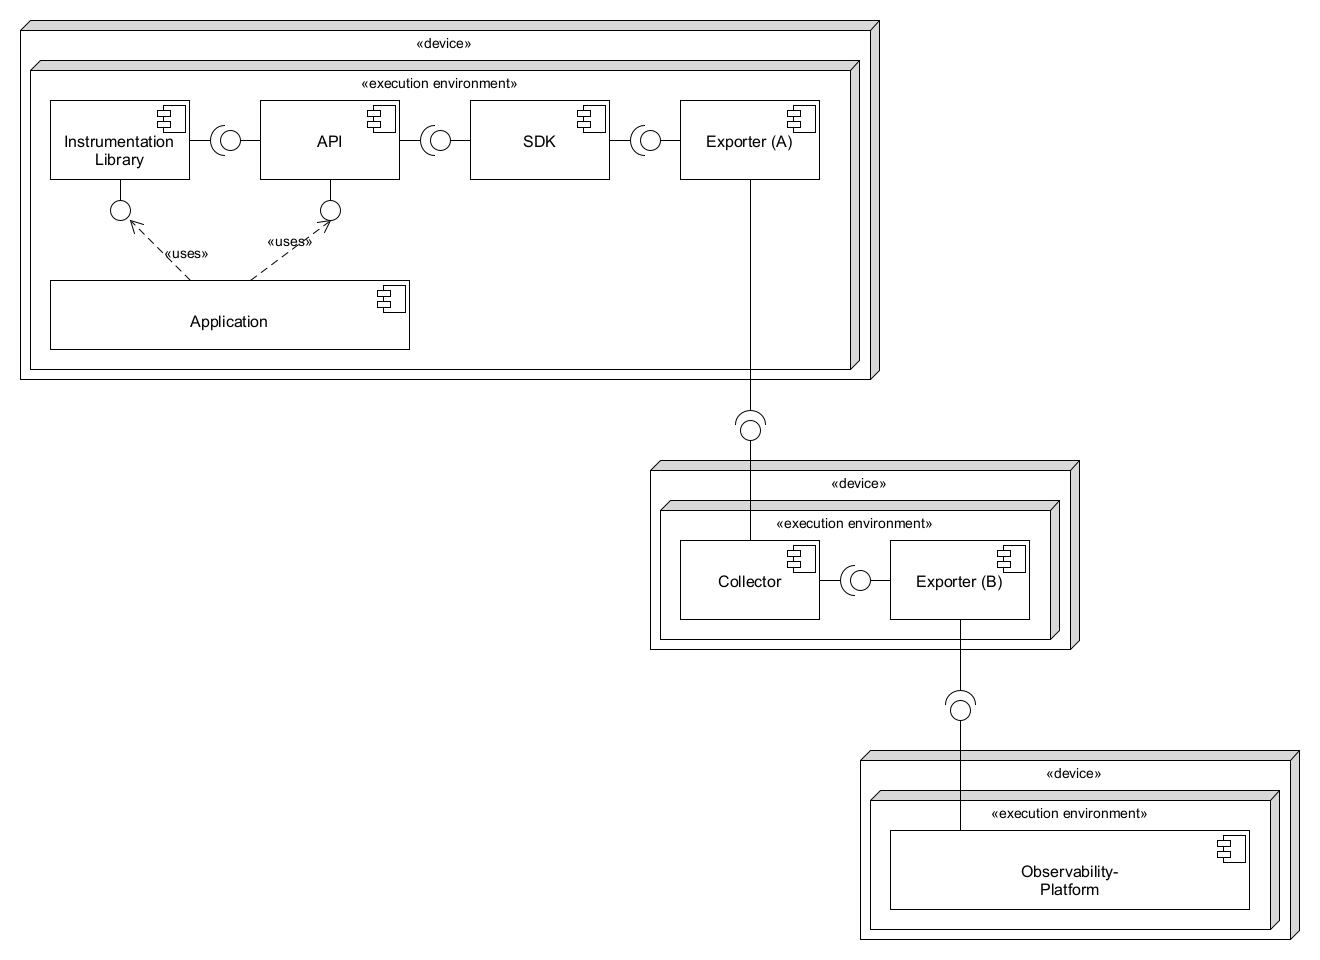
\includegraphics[width=1.00\linewidth]{img/03_methoden/otel_components.png}
	\caption{Komponenten von OpenTelemetry, eigene Darstellung auf Basis von \cite{OTelSpecification}}
	\label{fig:otel-components}
\end{figure}